

\chapter{Application to superconductivity}


In this chapter, we will study superconductivity which is one of the most remarkable physical phenomenon.

We first review the fundamental physical properties of superconductors.

We then introduce the BCS theory, which is one of the most successful application of quantum many-body techniques.

In terms of the BCS theory, we will see how all the fundamental superconducting properties can be understood from the microscopic point of views.



\section{Superconducting properties and thermodynamics relations}


Resistivity in metals decreases when the temperature goes down (See Fig{\ref{Fig6.1}}).

\begin{figure}
\begin{center}
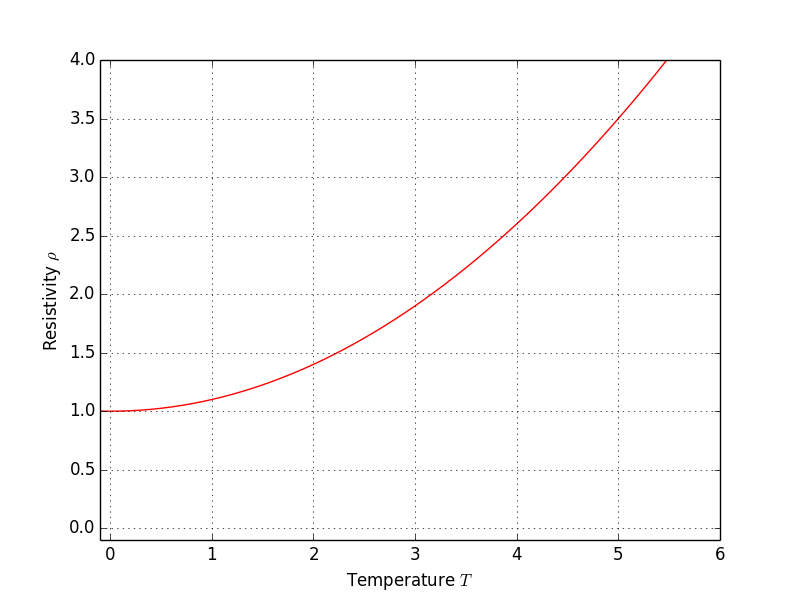
\includegraphics[width = 8cm]{6-1.png}\label{Fig6.1}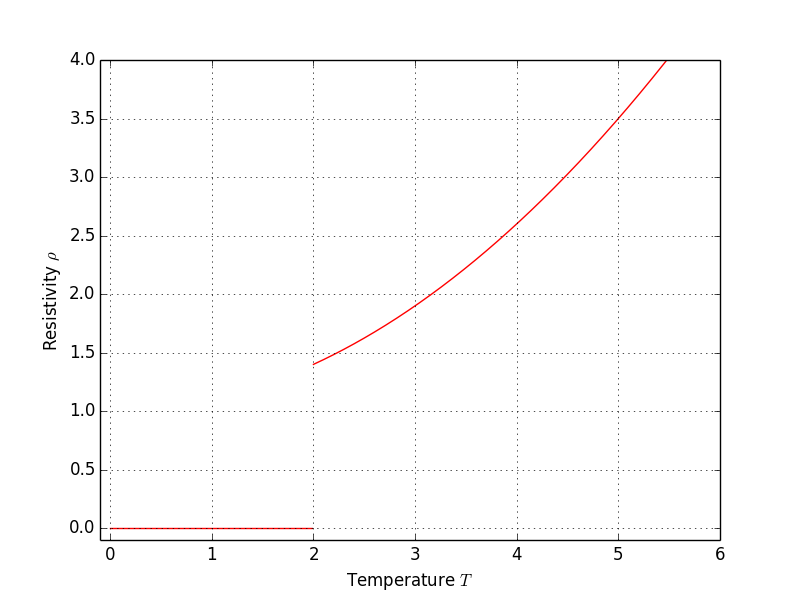
\includegraphics[width = 8cm]{6-2.png}\label{Fig6.2}
\caption{Resistivity $\rho$ vs. Temperature $T$ by $\rho = \rho_{res} + aT^2$ where `res' denotes residual resistivity. } \caption{Resistivity of superconductor's $\rho$ vs. Temperature $T$ by $\rho = \rho_{res} + aT^2$ where `res' denotes residual resistivity. } 
\end{center}
\end{figure}
The temperature dependence always exhibits $T^2$ behavior while the resistivity at the zero temperature remains finite, which we call residual resistivity $\rho_{res}$.
    
This residual resistivity stems from the scattering of conduction electron due to randomly distributed impurity and lattice defects. 
    
On the other hand, $T^2$-dependence of the resistivity comes from the scattering of conduction electrons due to electron-phonon interaction and electron-electron interactions. 
    
But, in some cases, metals exhibits an electronic phase transition at lower temperatures and resistivity becomes zero. 

The low-temperature phase with zero resistivity is called superconductor, or ``superconducting phase''. 

Simple-substance metals that exhibits superconductivity at lower temperature or under high pressure are shown in the following periodic table, where ``black-shaded'' simple substance metals show superconductivity (at lower temperature, $\blacksquare$ , while at lower temperature and under higher pressure, $\blacktriangle$ )

You might as well regard that in a sufficiently clean metal, the resistivity goes to zero at the zero-temperature, which we call ``perfect conductor'' instead of ``superconductor'', the electric conductivity diverges, so that the electric field $\mathscr{E}$ vanish inside the materials 

\noindent $(\bm{j} = \sigma \bm{E}) $

Then, the Maxwell equation tells us that the magnetic field {\uuline{subsequently}} applied after the system reach the zero-temperature will remains zero inside the material. 

\[\frac{\partial \bm{B}}{\partial t} = -c\ \text{rot}\bm{E} \]

because, during the application of the external fields, the electric field $\bm{E}$ remains zero inside the materials. 

Accordingly, both the perfect conductor at the zero-temperature and the superconductor ``expels'' the external magnetic field, when the fields are applied {\uuline{subsequently}} after the system reaches the zero-temperature. 

Remember that his is the case when the field is applied, after the temperature reaches zero-temperature. 

But, when we reduces the temperature under a finite external magnetic field, this is {\uuline{no longer}} the case for the ``perfect conductor'', while, this is still the case for the ``superconductor''. 

Namely: 

This exclusive of the magnetic field in the {\uuline{field-cooled superconductor}} s called as ``Meissner effect'', which is more essential ``\uwave{defining property}'' of superconductors than ``the zero-resistivity''. 

The ``Meissner effect'' can be understood from a phenomenological equation called London equation: 

\[\bm{j} = -\frac{ne^2}{mc}\bm{A} \]

where $\bm{j}$ is the current density and $\bm{A}$ is the vector potential. 

This equation can be roughly understtod by the following argument. 

In the superconductor, the electric current flow {\uuline{without any resistivity}}, so that we might as well begin with the newton's equation {\uuline{without dissipation}}: 

\[m\ddot{\bm{r}} = -e\bm{E} \]

Now that the current density is proportional to the velocity of electron

\[\bm{j} = -ne\dot{\bm{r}} \]

we might as well naively relate the time-derivative of the current with the electric field: 

\[\frac{d\bm{j}}{dt} = -\frac{ne^2}{m}\bm{E} = -\frac{ne^2}{mc}\frac{d\bm{A}}{dt} \]

Now that the electric field is given by the time-derivative of the vector potential, we might as well regard that the current is proportional to the vector potential

\[\bm{j} = -\frac{ne^2}{mc}\bm{A} \]

This London equation is, however, more or less a phenomenological equationand we will later see more microscopic derivation of this equation based on the BCS theory. 

Thereby, we will see that this equation holds true for a so-called Cooper pair, which is composed of two electrons, so that, the electron number density ``$n$'' is replaced by superelectron number density ``$n_s$''. 

\[\bm{j} = -\rho\cdot 2e \cdot\dot{\bm{r}} = -n_s e \dot{\bm{r}}\quad \text{where $\rho$ is the number of cooper pairs. } \]

In any case, this single phenomenological equation captures many important electromagnetic properties including Meissner effect. 

For example, the Meissner effect can be derived from the London equation as follows: 

From the Maxwell equation: 

\[\text{rot} \bm{B} = \frac{1}{c}\frac{\partial \bm{E}}{\partial t} + \frac{4\pi}{c}\bm{j} \]

we consider the temporally static situation: 

\[\text{rot}\bm{B} = \frac{4\pi}{c}\bm{j} = -\frac{4\pi ne^2}{mc^2}\bm{A}^t \]

Now $\bm{B} = \text{rot}\bm{A}$, we have

\[\text{rot\ rot}\bm{B} = -\frac{4\pi ne^2}{mc^2}\text{rot}\bm{A}^t \]
\[-\left(\nabla^2\vec{\bm{B}} - \nabla (\underset{=0}{\nabla \cdot \vec{\bm{B}}})\right) = -\frac{4\pi ne^2}{mc^2}\vec{\bm{b}} \]

\begin{align} \tag{A}
\Rightarrow \nabla^2 \bm{B} = \frac{4\pi ne^2}{mc^2}\bm{B} = \frac{1}{\lambda^2}\bm{B},\quad \lambda \equiv \sqrt{\frac{mc^2}{4\pi ne^2}} 
\end{align}

In order to solve this equation, let us consider a specific geometry of the superconducting material, so that we can define the boundary condition: 

Consider that the system is the salb geometry which has two parallel planes boundaries at $x = -L/2$ and at $x = L/2$. For simplicity, we assume that the system is infinitely large along $y,\, z$ -direction. We suppose $L$ to be very large. 

We apply the external field along $z$ direction: 

\[\begin{split}
\bm B\left(x < -\frac{L}{2}\right) &= B\hat{e}_z\\
\bm B\left(x > \frac{L}{2}\right) &= B\hat{e}_z
\end{split} \]

Now that the tangential component of $\bm{B}$ should be continuous at the two boundaries (at $x = \pm L/2$)







\section{BCS theory, Cooper pairing and Gap equation}

\subsection{BCS(Bardeen Copper Schrieffer) Hamiltonian}



Based on the experimental observation of the isotope effect, many people in 1950s had worked on the effect of electron-phonon interaction. 

As we have seen in the Section {\ref{se5-2}}, the electron-phonon coupled field theory is equivalent to the electron system with the attractive electron-electron interaction, so that we begin with the following simplified Hamiltonian called as the BCS Hamiltonian: 

\[\begin{split}
\hat{K} =& \hat{K}_0 + \hat{V} = \int d^3 \bm{x} \psi^{\dagger}_{\alpha}(\bm{x})\left[\frac{1}{2m}\left(-i\hbar \nabla + \frac{e\bm{A}(\bm{x})}{c}\right)^2-\mu\right]\psi_{\alpha}(\bm{x})\\
&-\frac{g}{2}\int d^3\bm{x}\psi^{\dagger}_{\alpha}(\bm{x})\psi^{\dagger}_{\beta}(\bm{x})\psi_{\beta}(\bm{x})\psi_{\alpha}(\bm{x})
\end{split} \]

where $\bm{A}(\bm{x})$ is a vector potential. 

Prior to the BCS theory, Cooper had considered two-electrons problem, which are introduced into a Fermi sea and which are interacting with each other via the attractive interaction. 

Without the attractive interaction, the energy cost we need to pay for these creations is 

\[\Delta E = \frac{\hbar k_1^2}{2m} + \frac{\hbar k_2^2}{2m}-2\mu > 0 \]

which is positive (so that the metal is stable). 

Cooper showed that, once the {\uuline{small}} attractive interaction between these two are introduced, the energy ``\uuline{cost}'' for the creating this pari of fermions near the Fermi surface becomes ``\uuline{negative}'', due to the binding energy. 

between these two particles, 

\[\Delta E = \frac{\hbar k_1^2}{2m} + \frac{\hbar k_2^2}{2m}-2\mu < 0 \]

This means that, once the attractive interaction are introduced near the Fermi surface, which is indeed the case with the ``effective'' BCS Hamiltonian, the Fermi sea (the ground state wave function for normal metal) is \uuline{stable} toward the formations of many pairs of fermions which are bound together by the attractive interaction. 

However, Cooper also showed that a finite binding energy between the two fermions comes from the Pauli exclusion due to the background Fermi-sea state. 

Therefore, the ``true'' ground state which we would obtain from the Fermi-sea state is NOT just a pure state of many bound pairs. 

Instead, the true ground state is \uwave{a linear superposition of those states having different number of the bound pairs}. 

\begin{align}\tag{A} \label{eqA}
|\Psi\rangle = |N-\text{particle}\rangle + |(N+2)-\text{particle}\rangle + |(N+4)-\text{particle}\rangle + \cdots + |(N+2m)-\text{particle}\rangle + \cdots \end{align}

Contrary to the ground state wavefunction for the normal phase, such a wave function gives a finite expectation value of the square of the creation fields: 

\[\begin{split}
\langle \Psi|\psi^{\dagger}\psi^{\dagger}|\Psi\rangle =& \langle (N+2)-\text{particle}|\psi^{\dagger}\psi^{\dagger}|N-\text{particle}\rangle \\ &+ \langle(N+4)-\text{particle}|\psi^{\dagger}\psi^{\dagger}|(N+2)-\text{particle}\rangle\\ & + \cdots \neq 0 \end{split}\]

In fact, we will see that the BCS ground state wavefunction is given by this type linear superposition where each of these multiparticle states have a phase coherence

\[|\Psi\rangle = e^{i\phi_N}|N-\text{particle}\rangle + e^{i\phi_{N+2}}|(N+2)-\text{particle}\rangle + e^{i\phi_{N+4}}|(N+4)-\text{particle}\rangle + \cdots  \]

where $\phi_M$ are \uline{not} randomly distributed in $M$. 

Based on this observation, BCS regards $\langle\psi^{\dagger}\psi^{\dagger}\rangle$ (or $\langle \psi\psi\rangle$) as an order-parameter for the superconductivity, and construct the Mean-field theory for $\langle \psi^{\dagger}\psi^{\dagger}\rangle$. 

The BCS Hamiltonian reads 

\[\begin{split}\hat{K}& = \int d^3 \bm{x}\psi^{\dagger}_{\alpha}(\bm{x})\left(-\frac{\hbar^2\nabla^2}{2m} - \mu\right)\psi_{\alpha}(\bm{x})\\
&-\frac{1}{2} \int d^3\bm{x} \hat{\psi}_{\alpha}^{\dagger}(\bm{x}) \hat{\psi}_{\beta}^{\dagger}(\bm{x}) \hat{\psi}_{\beta}(\bm{x})\hat{\psi}_{\alpha}(\bm{x}) \end{split}\]

where the interaction part can be rewritten into 

\[\begin{split}\psi_{\alpha}^{\dagger}(\bm{x})\psi_{\beta}^{\dagger}(\bm{x})&\psi_{\beta}(\bm{x})\psi_{\alpha}(\bm{x})\\
 &=  \left(\langle\psi^{\dagger}_{\alpha}(\bm{x})\psi^{\dagger}_{\beta}(\bm{x})\rangle + \psi^{\dagger}_{\alpha}(\bm{x})\psi^{\dagger}_{\beta}(\bm{x}) - \langle\psi^{\dagger}_{\alpha}(\bm{x})\psi^{\dagger}_{\beta}(\bm{x})\rangle\right)\\
&\times \left(\langle\psi_{\beta}(\bm{x})\psi_{\alpha}(\bm{x})\rangle + \psi_{\beta}(\bm{x})\psi_{\alpha}(\bm{x}) - \langle\psi_{\beta}(\bm{x})\psi_{\alpha}(\bm{x})\rangle\right)
\end{split}\]

Suppose that the fluctuation from the mean-field ($\psi^{\dagger}_{\alpha}(\bm{x})\psi^{\dagger}_{\beta}(\bm{x}) - \langle\psi^{\dagger}_{\alpha}(\bm{x})\psi^{\dagger}_{\beta}(\bm{x})\rangle$) is small; we ignore the quadratic in the fluctuation: 

\[\begin{split}
\left(\psi^{\dagger}_{\alpha}(\bm{x})\psi^{\dagger}_{\beta}(\bm{x}) - \langle\psi^{\dagger}_{\alpha}(\bm{x})\psi^{\dagger}_{\beta}(\bm{x})\rangle\right)\\
\times \left(\psi_{\alpha}(\bm{x})\psi_{\beta}(\bm{x}) - \langle\psi_{\alpha}(\bm{x})\psi_{\beta}(\bm{x})\rangle\right) \rightarrow 0\end{split}\]

The other terms are summarized as 

\[\begin{split}
 =&\psi^{\dagger}_{\alpha}(\bm{x})\psi^{\dagger}_{\beta}(\bm{x})\langle\psi_{\alpha}(\bm{x})\psi_{\beta}(\bm{x})\rangle\\
& + \langle\psi^{\dagger}_{\alpha}(\bm{x})\psi^{\dagger}_{\beta}(\bm{x})\rangle\psi_{\alpha}(\bm{x})\psi_{\beta}(\bm{x}) - \langle\psi^{\dagger}_{\alpha}(\bm{x})\psi^{\dagger}_{\beta}(\bm{x})\rangle\langle\psi_{\alpha}(\bm{x})\psi_{\beta}(\bm{x})\rangle \end{split} \]

from which we obtain a mean-field Hamiltonian 

\[\begin{split}\hat{K}_{eff} =& \hat{K}_0 - \frac{g}{2} \int d^3 \bm{x} \left\{\langle\psi^{\dagger}_{\alpha}(\bm{x})\psi^{\dagger}_{\beta}(\bm{x})\rangle\psi_{\beta}(\bm{x})\psi_{\alpha}(\bm{x}) +\psi^{\dagger}_{\alpha}(\bm{x})\psi^{\dagger}_{\beta}(\bm{x}) \langle\psi_{\beta}(\bm{x})\psi_{\alpha}(\bm{x})\rangle\right\} + \text{const}\\
=& \hat{K}_0 - \frac{g}{2} \int d^3 \bm{x} \left\{\langle\psi^{\dagger}_{\uparrow}(\bm{x})\psi^{\dagger}_{\downarrow}(\bm{x})\rangle\psi_{\downarrow}(\bm{x})\psi_{\uparrow}(\bm{x}) +\langle\psi_{\downarrow}(\bm{x})\psi_{\uparrow}(\bm{x})\rangle\psi^{\dagger}_{\uparrow}(\bm{x})\psi^{\dagger}_{\downarrow}(\bm{x}) \right\} + \text{const}\\
 =&\hat{K}_0 - g\int d^3\bm{x} \left\{\langle\psi_{\downarrow}(\bm{x})\psi_{\uparrow}(\bm{x})\rangle\psi^{\dagger}_{\uparrow}(\bm{x})\psi^{\dagger}_{\downarrow}(\bm{x}) +\psi_{\downarrow}(\bm{x})\psi_{\uparrow}(\bm{x})\langle\psi^{\dagger}_{\uparrow}(\bm{x})\psi^{\dagger}_{\downarrow}(\bm{x})\rangle \right\}\\
&+g\int d^3 \bm{x} \langle\psi^{\dagger}_{\downarrow}(\bm{x})\psi^{\dagger}_{\uparrow}(\bm{x})\rangle \langle\psi_{\uparrow}(\bm{x})\psi_{\downarrow}(\bm{x})\rangle
 \end{split}\]

In order to make the theory self-consistent, we assume that the mean-field is given by the expectation value of the product of the creation fields, \uwave{calculated with respect to the ground state wavefunction for mean-field Hamiltonian}:

\[\langle\psi_{\downarrow}^\dagger(\bm{x})\psi_\uparrow^\dagger(\bm{x})\rangle \equiv \langle\Phi_0|\psi_\uparrow^\dagger(\bm{x})\psi_\uparrow^\dagger(\bm{x})|\Phi_0\rangle \]

where $|\Phi_0\rangle$ is the ground state w.f for $\hat{K}_{eff}$. 

\[
\begin{split}
\hat{K}_{eff}&=\int d^3\bm{x}\psi_\alpha^\dagger(\bm{x})\left(-\frac{\hbar^2\nabla_{\bm{x}}^2}{2m}-\mu\right)\psi_\alpha(\bm{x})\\
&-g\int d^3\bm{x}\{\langle\psi_\downarrow^\dagger(\bm{x})\psi_\uparrow^\dagger(\bm{x})\rangle \psi_\uparrow(\bm{x})\psi_\downarrow(\bm{x})\\
&\quad+\psi_\downarrow^\dagger(\bm{x})\psi_\uparrow^\dagger(\bm{x}) \langle\psi_\uparrow^\dagger(\bm{x})\psi_\downarrow^\dagger(\bm{x})\rangle\}\\
&+g\int d^3\bm{x}\langle\psi_\downarrow^\dagger(\bm{x})\psi_\uparrow^\dagger(\bm{x})\rangle \underset{-\Delta(\bm{x})}{\uwave{\langle\psi_\uparrow(\bm{x})\psi_\downarrow(\bm{x})\rangle}}
\end{split}
 \]

Provided that the ground state wavefunction does not break the translational symmetry spontaneously, we can regard that the mean-field does not depends on the space coordinate. 

\[g\langle\psi_\downarrow^\dagger(\bm{x})\psi_\uparrow^\dagger(\bm{x})\rangle \equiv-\Delta^*\equiv|\Delta|e^{-i\theta} \]

With this in mind, the mean-field Hamiltonian is readily diagonalized:

\[\begin{split}
\hat{K}_{eff} &=\sum_{\bm{k}, \alpha}\left(\overset{\xi_{\bm{k}}}{\frac{\hbar^2\bm{k}^2}{2m}}-\mu\right)c_{\bm{k},\alpha}^\dagger c_{\bm{k},\alpha}\\
&+\Delta^* \sum_{\bm{k}} c_{\bm{k}\uparrow}c_{-\bm{k}\downarrow}+ \Delta\sum_{\bm{k}}c_{-\bm{k}\downarrow}^\dagger c_{\bm{k}\uparrow}^\dagger - \Delta\sum_{\bm{k}}\langle c_{-\bm{k}\downarrow}^\dagger c_{\bm{k}\uparrow}^\dagger\rangle\\
&=\sum_{\bm{k}}\left\{(c_{\bm{k}\uparrow}^\dagger\  c_{-\bm{k}\downarrow}) \left(\begin{matrix}
\xi_{\bm{k}} & -e^{i\theta}|\Delta|\\
-e^{-i\theta}|\Delta| & -\xi_{\bm{k}}
\end{matrix}\right)
\left(\begin{matrix}
c_{\bm{k}\uparrow}\\
c_{-\bm{k}\downarrow}^\dagger
\end{matrix}\right)+\xi_{\bm{k}}\right\}-\Delta\sum_{\bm{k}}\langle c_{-\bm{k}\downarrow}^\dagger c_{\bm{k}\uparrow}^\dagger\rangle
\end{split} \]

A unitary transformation gives

\[
\left(\begin{matrix}
c_{\bm{k}\uparrow}\\
\ \\
c_{-\bm{k}\downarrow}^\dagger
\end{matrix}\right) 
= \left(\begin{matrix}
u_k & e^{i\theta}v_k\\
\ & \ \\
-e^{-i\theta}v_k & u_k
\end{matrix}\right) \left(\begin{matrix}
\alpha_{\bm{k}}\\
\ \\
\beta_{-\bm{k}}^\dagger
\end{matrix}\right)  \]

with

\[
\begin{cases}
2u_{\bm{k}}v_{\bm{k}} &= \displaystyle\frac{|\Delta|}{\sqrt{\xi_{\bm{k}}^2+|\Delta|^2}}\\
\ & \ \\
u_{\bm{k}}^2-v_{\bm{k}}^2 &= \displaystyle\frac{\xi_{\bm{k}}}{\sqrt{\xi_{\bm{k}}^2+|\Delta|^2}}
\end{cases}\]

Or equivalently

\[
\begin{cases}
u_{\bm{k}} &= \displaystyle\frac{1}{\sqrt{2}}\left(1+\frac{\xi_{\bm{k}}}{\sqrt{\xi_{\bm{k}}^2+|\Delta|^2}}\right)^{1/2}\\
\ & \ \\
v_{\bm{k}} &= \displaystyle\frac{1}{\sqrt{2}}\left(1-\frac{\xi_{\bm{k}}}{\sqrt{\xi_{\bm{k}}^2+|\Delta|^2}}\right)^{1/2}
\end{cases}
\]

In terms of this, we have

\[\begin{split}
\hat{K}_{eff}&=\sum_{\bm{k}}\left\{\sqrt{\xi_{\bm{k}}^2+|\Delta|^2}(\alpha_{\bm{k}}^\dagger(\alpha_{\bm{k}}-\beta_{-\bm{k}}\beta_{-\bm{k}}^\dagger)+\xi_{\bm{k}}\right\}- \Delta\sum_{\bm{k}}\langle c_{-\bm{k}\downarrow}^\dagger c_{\bm{k}\uparrow}^\dagger\rangle\\
&= V+\sum_{\bm{k}}\sqrt{\xi_{\bm{k}}^2+|\Delta|^2}(\alpha_{\bm{k}}^\dagger\alpha_{\bm{k}}+\beta_{\bm{k}}^\dagger\beta_{\bm{k}}
\end{split}\]

where

\[V \equiv\sum_{\bm{k}}\{\xi_{\bm{k}}-\sqrt{\xi_{\bm{k}}^2+|\Delta|^2}-\Delta\langle c_{-\bm{k}\downarrow}^\dagger c_{\bm{k}\uparrow}^\dagger\rangle\} \]

Now that $\hat{K}_{eff}$ is given by a quadratic form in the creation fields $(\alpha_{\bm{k}}^\dagger, \beta_{\bm{k}}^\dagger)$ and annihilation fields $(\alpha_{\bm{k}}, \beta_{\bm{k}})$, the eigen state of $\hat{K}_{eff}$ is given by a multi particle state of these new quasic particle. 

Noting that these fields as well as the original fields $(c_{\bm{k},\sigma}, c_{\bm{k},\sigma}^\dagger)$ are fermion fields, the eigen state is given by 

\[|(\bm{k}_1,\alpha_1),\cdots,(\bm{k}_n\beta)\rangle = \alpha_{\bm{k}_1}^\dagger \cdots \beta_{\bm{k}_n}^\dagger|\Phi_0\rangle \]

where $|\Phi_0\rangle$ denotes the vacuum of $\alpha$-particle and $\beta$-particle (called as Bogoliubov particles). 

\[\begin{cases}
\alpha_{\bm{k}}|\Phi_0\rangle &= 0\\
\ & \ \\
\beta_{\bm{k}}|\Phi_0\rangle &= 0
\end{cases}\]

Since creating the Bogoliubov particles is always accompanied by a positive energy $(\sqrt{\xi_{\bm{k}}^2+|\Delta|^2}>0$, the vacuum is nothing but the ground state wavefunction of $\hat{K}_{eff}$, whose energy is $V$. 

\[\hat{K}_{eff}|\Phi_0\rangle = \overset{\sum_{\bm{k}}\xi_{\bm{k}}-\sqrt{\xi_{\bm{k}}^2+|\Delta|^2}-\Delta\langle c_{-\bm{k}\downarrow}^\dagger c_{\bm{k}\uparrow}^\dagger\rangle}{\quad\quad\quad\quad\quad\quad\quad\quad\quad\quad\quad V}|\Phi_0\rangle \]

A group of the lowest excited states is given by ``one-particle'' state of the Bogoliubov particle

\[\begin{split}
\alpha_{\bm{k}}^\dagger|\Phi_0\rangle &= |\bm{k},\alpha\rangle\\
\beta_{\bm{k}}^\dagger|\Phi_0\rangle &= |\bm{k}, \beta\rangle
\end{split}\]

\[\hat{K}_{eff} \alpha_{\bm{k}}^\dagger|\Phi_0\rangle = (V+\sqrt{\xi_{\bm{k}}^2+|\Delta|^2})\alpha_{\bm{k}}^\dagger|\Phi_0\rangle \]

which is a \uline{gapped} excitation (See Fig. \ref{Fig6.3}) because of $\sqrt{\xi_{\bm{k}}^2+|\Delta|^2}\ge|\Delta|$. 

\begin{figure}
\begin{center}
\begin{tikzpicture}
\draw [red] (0,0.9) -- (4,0.9);
\draw [dashed] (0,1.9) -- (2,1.9);
\draw (0,3) arc [start angle=-150, end angle=-30, radius=2.2];
\draw [->](-0.3,0) -- (4,0);
\draw (4.5,0) node {$k$};
\draw [->](0, -0.3) -- (0,3.3);
\draw (0,3.8) node {$E$};
\draw (-0.5,1) node {$V$};
\draw (-1, 2) node {$V+|\Delta|$};
\draw [dashed] (2,1.9) -- (2,0);
\draw (2,-0.5) node {$k_0 = {\bf{k}}-k_F$};
\end{tikzpicture}
\end{center}
\caption{Excited spectrum; red line for ground BCS state, and solid line for single excited state; $k_0$ stands for $\xi_{k_0} = 0$. }\label{Fig6.3}
\end{figure}

This gapped behaviour of the one-particle excitation of the Bogoliubov particle is the origin of the thermal activation form of the low-temperature specific heat in superconductors. (see later)

To see the mean-field ground state wavefunction thus introduced indeed take the form of eq. \ref{eqA}, let us construct the $|\Phi_0\rangle$ in terms of the original (electron) creation and annihilation operators: 

Now that $\alpha_{\bm{k}}$ and $\beta_{\bm{k}}$ are given by a linear combination of $c_{\bm{k}\uparrow}$ and $c_{-\bm{k}\downarrow}^\dagger$

\[
\left(\begin{matrix}
\alpha_{\bm{k}}\\
\ \\
\beta_{-\bm{k}}^\dagger
\end{matrix}\right) = \left(\begin{matrix}
u_{\bm{k}} & -e^{i\theta}v_{\bm{k}}\\
\ & \ \\
e^{-i\theta}v_{\bm{k}} & u_{\bm{k}}
\end{matrix}\right) \left(\begin{matrix}
c_{\bm{k}\uparrow}\\
\ \\
c_{-\bm{k}\downarrow}^\dagger
\end{matrix}\right) 
 \]

or

\[\alpha_{\bm{k}} = u_{\bm{k}}c_{\bm{k}\uparrow} - e^{i\theta}v_{\bm{k}}c_{-\bm{k}\downarrow}^\dagger \]
\[\beta_{-\bm{k}} = e^{i\theta}v_{\bm{k}}c_{\bm{k}\uparrow}^\dagger + u_{\bm{k}}c_{-\bm{k}\downarrow} \]
\[(\beta_{\bm{k}} = e^{i\theta}v_{\bm{k}}c_{-\bm{k}\uparrow}^\dagger+u_{\bm{k}}c_{\bm{k}\downarrow}) \]

This vacuum of such Bogoliubov particles given by: \footnote{This solution is derived based on guess, not rigorous calculation. The following shows some check for this solution. }

\[|\Phi_0\rangle = \prod_{\bm{k}}(u_{\bm{k}}+e^{i\theta}v_{\bm{k}}c_{\bm{k}\uparrow}^\dagger c_{-\bm{k}\downarrow}^\dagger)|vac\rangle \]

where $|vac\rangle$ denotes the vacuum of the original electrons ($c_{\bm{k}\sigma}|vac\rangle = 0$ for $\forall\ \bm{k},\sigma$) and the product over $\bm{k}$ is taken over all momentum. 

In fact, one can see that 

\[
\begin{split}
\alpha_{\bm{k}'}|\Phi_0\rangle &= \prod_{\bm{k} \neq \bm{k}'} (u_{\bm{k}}+e^{i\theta}v_{\bm{k}}c_{\bm{k}\uparrow}^\dagger c_{-\bm{k}\downarrow}^\dagger)\times( u_{\bm{k}'}c_{\bm{k}'\uparrow} - e^{i\theta}v_{\bm{k}'}c_{-\bm{k}'\downarrow}^\dagger)(u_{\bm{k}'}+e^{i\theta}v_{\bm{k}'}c_{\bm{k}'\uparrow}^\dagger c_{-\bm{k}'\downarrow}^\dagger)|vac\rangle \\
&=\prod_{\bm{k}\neq\bm{k}'}(u_{\bm{k}}+e^{i\theta}v_{\bm{k}}c_{\bm{k}\uparrow}^\dagger c_{-\bm{k}\downarrow}^\dagger)\\
&\ \ \times (u_{\bm{k}'}^2c_{\bm{k}'\uparrow}+e^{i\theta}u_{\bm{k}'}v_{\bm{k}'}(1-c_{\bm{k}'\uparrow}^\dagger c_{\bm{k}'\uparrow})c_{-\bm{k}'\downarrow}^\dagger\\
&\quad\quad -e^{i\theta}u_{\bm{k}'}v_{\bm{k}'}c_{-\bm{k}'\downarrow}^\dagger + e^{i\theta}v_{\bm{k}'}^2c_{\bm{k}'\uparrow}^\dagger(c_{-\bm{k}'\downarrow}^\dagger)^2)|vac\rangle\\
&=0
\end{split}\]

Similar for applying $\beta_{\bm{k}'}$ on this and obviously derive a $0$ as well. 

Then, the many body wavefunction is given by ``a linear superposition of those states having different but even numbers of electrons''. 

\[|\Phi_0\rangle = |vac\rangle + |2-\text{particle}\rangle + |4-\text{particle}\rangle+\cdots \]

so that the expectation value of the product of two creation fields can be finite. 

To calculate $\langle\psi_{\downarrow}(\bf{x})^\dagger\psi_{\downarrow}(\bf{x})^\dagger\rangle$, notice first that $|\Phi_0\rangle$ is already normalized

\[\begin{split}
\langle\Phi_0|\Phi_0\rangle &= \langle vac| \prod_{\bm{k}}\{(u_{\bm{k}}+e^{-i\theta}v_{\bm{k}}c_{-\bm{k}\downarrow}c_{\bm{k}\uparrow})(u_{\bm{k}}+e^{i\theta}v_{\bm{k}}c_{\bm{k}\uparrow}^\dagger c_{-\bm{k}\downarrow}^\dagger)\}|vac\rangle\\
&= \langle vac|\prod\{u_{\bm{k}}^2+v_{\bm{k}}^2c_{-\bm{k}\downarrow}\underset{=1-c_{\bm{k}\uparrow}^\dagger c_{\bm{k}\uparrow}}{c_{\bm{k}\uparrow}c_{\bm{k}\uparrow}^\dagger} c_{-\bm{k}\downarrow}^\dagger\}|vac\rangle\\
&=\langle vac|vac\rangle = 1
\end{split}\]

Thus the mean-field is readily calculated as follows: %Page 952

\[\begin{split}
\langle\psi_{\downarrow}(\bm{x})^\dagger\psi_{\uparrow}(\bm{x})^\dagger\rangle &= \frac{1}{V}\int d^3 \bm{x} \langle\psi_{\downarrow}(\bm{x})^\dagger\psi_{\uparrow}(\bm{x})^\dagger\rangle = \frac{1}{V} \sum_{\bm{k}}\langle\Phi_0|c_{-\bm{k}\downarrow}^\dagger c_{\bm{k}\uparrow}^\dagger|\Phi_0\rangle \\
&\quad\text{left hand side is independent of }\bm{x}\\
&= \frac{1}{V}\sum_{\bm{k}}\langle vac|(u_{\bm{k}}+e^{-i\theta}v_{\bm{k}}c_{-\bm{k}\downarrow}c_{\bm{k}\uparrow})c_{-\bm{k}\downarrow}^\dagger c_{\bm{k}\uparrow}^\dagger (u_{\bm{k}}+e^{i\theta}v_{\bm{k}}c_{\bm{k}\uparrow}^\dagger c_{-\bm{k}\downarrow}^\dagger)|vac\rangle\\
&= -\frac{1}{V}e^{-i\theta}\sum_{\bm{k}}v_{\bm{k}}u_{\bm{k}}
\end{split}\]

Multiply $g$ and substitute the expressions for $u_{\bm{k}}, v_{\bm{k}}$ in terms of $\Delta$, we obtain

\[|\Delta| = \frac{g}{2}\int \frac{d^3 \bm{k}}{(2\pi)^3}\frac{|\Delta|}{\sqrt{\xi_{\bm{k}}^2+|\Delta|^2}} \]

which is called a ``gap equation'', determine $|\Delta|$. 

Remember that the attraction interaction in the BCS Hamiltonian applies for those two electrons which are lying within an energy shell of the thickness $\hbar \omega_D$ from the Fermi surface (see previous argument).

This restriction tells us that $\hat{K}_{eff}$ with finite $|\Delta|$ holds true only for those momentum $\bm{k}$, which satisfy

\[|\xi_{\bm{k}}| \equiv |\frac{\hbar^2 \bm{k}^2}{2m}-\mu|<\hbar \omega_D \]

For the other $\bm{k}$, the off-diagonal term connecting $c_{\bm{k}\uparrow}$ and $c_{-\bm{k}\downarrow}$ should be set to zero:

\[\hat{K}_{eff}=\sum_{\bm{k},\alpha}\xi_{\bm{k}}c_{\bm{k}\alpha}^\dagger c_{\bm{k}\alpha}+\Delta^* \sum_{\bm{k},|\xi_{\bm{k}}|<\hbar\omega_D}c_{\bm{k}\uparrow}c_{-\bm{k}\downarrow}+\Delta\sum_{\bm{k},|\xi_{\bm{k}}|<\hbar\omega_D}c_{-\bm{k}\downarrow}^\dagger c_{\bm{k}\uparrow}^\dagger \]

which leads to

\[\begin{cases}
 (u_{\bm{k}},v_{\bm{k}}) = (1,0)\text{ for }\xi_{\bm{k}}>\hbar\omega_D\\
\ \\
(u_{\bm{k}},v_{\bm{k}}) = (0,1)\text{ for }\xi_{\bm{k}}<-\hbar\omega_D
\end{cases}\]

Thus, the right hand side acquires a cut off:

\[|\Delta|=\frac{g}{2}\underset{|\xi_{\bm{k}}|\le\hbar\omega_D}{\int}\frac{d^3 \bm{k}}{(2\pi)^3}\frac{|\Delta|}{\sqrt{\xi_{\bm{k}}^2+|\Delta|^2}} \]

because

\[u_k v_k = \begin{cases}
\frac{\Delta}{\sqrt{\xi_k^2+|\Delta|^2}} & for\ |\xi_k|\le\hbar\omega_D\\
9 & for\ otherwise
\end{cases} \]

\dotfill

\ 

\[\int_{|\xi_k|\le\hbar\omega_D}\frac{d^3{\bf k}}{(2\pi)^2}f(\xi_k) = \frac{1}{V}\sum_{\bf k}f(\xi_k) = \int_{-\hbar\omega_D}^{\hbar\omega_D}d\omega f(\omega) {\color{red}{\frac{1}{V}\sum_{\bf k}\delta(\omega-\xi_k)}} \overset{def}{\equiv}\int_{-\hbar\omega_D}^{\hbar\omega_D}d\omega f(\omega) d\omega f(\omega)N(\omega) \]

\dotfill

\ 

\[\cancel{|\Delta|} = g\int_{-\hbar\omega_D}^{\hbar\omega_D}d\omega N(\omega)\frac{\cancel{|\Delta|}}{\sqrt{\omega^2+|\Delta^2|}} \]

In usual metal, characteristic frequency scale of $N(\omega)$ (e.g. band width) is much larger than the band width of the acoustic phonon ($\hbar\omega_D$). As such, one might as well replace $N(\omega)$ by the density of state at the chemical potential $N(0)$

\[\begin{split}
1 &= g\underset{\frac{mk_F}{2\pi^2\hbar^2}}{N(0)}\int_0^{\hbar\omega_D} d\omega\frac{1}{\sqrt{\omega^2+|\Delta|^2}} = gN(0)\left[\ln[\omega+\sqrt{\omega^2+|\Delta^2|}]\right]\Big|_0^{\hbar\omega_D}\\
&=gN(0)\ln\left[\frac{\hbar\omega_D+\sqrt{(\hbar\omega_D)^2+|\Delta^2|}}{|\Delta|}\right]\\
&\approx gN(0)\ln\left(\frac{2\hbar\omega_D}{\Delta}\right)\quad (\Delta\ll\hbar\omega_D)
\end{split} \]

\begin{align}\tag{B}
|\Delta| = 2\hbar\omega_De^{-\frac{1}{gN(0)}}
\end{align}

For typical metals, $N(0)g\approx0.2-0.3$ so that $|\Delta|$ can be induced regarded as much smaller than $\hbar\omega_D$. 

\dotfill

\ 

In order to generalize the BCS mean-field theory to {\uuline{a finite temperature}}, we have only to change the interpretation of $\langle\psi_{\downarrow}^\dagger({\bf x})\psi_{\uparrow}^\dagger({\bf x})$. 

Namely, the mean0field is now given by the ensemble average of the product of the creation field calculated with respect to $\hat{K}_{eff}$

\[\langle\psi_{\downarrow}^\dagger({\bf x})\psi_{\uparrow}^\dagger({\bf x}) = \frac{\trace[e^{-\beta\hat{K}_{eff}}\langle\psi_{\downarrow}^\dagger({\bf x})\psi_{\uparrow}^\dagger({\bf x})]}{\trace[e^{-\beta\hat{K}_{eff}]}} \]

As we will see below, the right hand side can be calculated in terms of \uline{the temperature Green's function} and it is given by the mean-field itself. 

To do this, let us first introduce the Heisenberg operator in the imaginary time;\footnote{For later convenience, we will introduce the external vector potential into the mean-field Hamiltonian
\[\hat{K}_{eff}=\int d^3{\bf x}\psi_{\alpha}^\dagger({\bf x})\left[\frac{1}{2m}\left(-i\hbar\nabla+\frac{e{\bf A}({\bf x})}{c}\right)^2-\mu\right]\psi_{\alpha}({\bf x}) - g\int d^3{\bf x}\{\langle\psi_{\downarrow}^\dagger({\bf x})\psi_{\uparrow}^\dagger({\bf x})\psi_{\uparrow}({\bf x})\psi_{\downarrow}({\bf x})+ h.c.\}+\cdots \]}

\[\begin{split}
\hat{\psi}_{k\uparrow}({\bf x},\tau) &= e^{\hat{K}_{eff}\tau/\hbar}\hat{\psi}_{\uparrow}({\bf x})e^{-\hat{K}_{eff}\tau/\hbar}\\
\hat{\psi}^\dagger_{k\downarrow}({\bf x},\tau) &= e^{\hat{K}_{eff}\tau/\hbar}\hat{\psi}^\dagger_{\downarrow}({\bf x})e^{-\hat{K}_{eff}\tau/\hbar}
\end{split} \]

which satisfy the following \uuline{linearized} equations of motions respectively:%956

Using these Heisenberg operators we next define the time-ordered Green's function

\[g({\bf x},\tau;{\bf x}',\tau') = -\langle T_{\tau}[\hat{\psi}_{k\uparrow}({\bf x},\tau)\hat{\psi}^\dagger_{k\uparrow}({\bf x}',\tau')]\rangle = -\theta(\tau-\tau')\langle\hat{\psi}_{k\uparrow}({\bf x},\tau)\hat{\psi}^\dagger_{k\uparrow}({\bf x}',\tau')\rangle + \theta(\tau'-\tau)\langle\hat{\psi}^\dagger_{k\uparrow}({\bf x}',\tau')\hat{\psi}_{k\uparrow}({\bf x},\tau)\rangle\]

Using the equations of motion for $\hat{\psi}_{k\uparrow}({\bf x},\tau)$, we can derive that for the Green's function

\[\begin{split}
\hbar\frac{\partial }{\partial t}g({\bf x},\tau;{\bf x'},\tau') &= -\hbar\delta(\tau-\tau')\langle\{\hat{\psi}_{k\uparrow}({\bf x},\tau),\hat{\psi}^\dagger_{k\uparrow}({\bf x}',\tau')\}\rangle - \langle \trace\left\{\hbar\frac{\partial \hat{\psi}_{k\uparrow}({\bf x},\tau)}{\partial \tau}\cdot\hat{\psi}_{k\uparrow}({\bf x}',\tau')^\dagger\right\}\rangle\\
&=-\hbar\delta(\tau-\tau')\langle\{\hat{\psi}_{k\uparrow}({\bf x},\tau),\hat{\psi}^\dagger_{k\uparrow}({\bf x}',\tau')\}\rangle + \left[\frac{1}{2m}\left(-i\hbar\nabla+\frac{e{\bf A}}{c}\right)^2-\mu\right]\langle\trace\{\hat{\psi}_{k\uparrow}({\bf x},\tau)\hat{\psi}^\dagger_{k\uparrow}({\bf x}',\tau')\}\rangle\\
&\phantom{=\ } + g\langle\psi_\uparrow({\bf x})\psi_{\downarrow}({\bf x})\langle\trace\{\hat{\psi}_{k\downarrow}({\bf x},\tau)\hat{\psi}^\dagger_{k\downarrow}({\bf x}',\tau')\}\rangle\\
&=-\hbar\delta(\tau-\tau')\delta^3({\bf x-x}') + \left[\frac{1}{2m}\left(-i\hbar\nabla+\frac{e{\bf A}}{c}\right)^2-\mu\right]\langle T_\tau \{\psi_{k\uparrow}({\bf x},\tau)\psi^\dagger_{k\uparrow}({\bf x'},\tau')\}\rangle\\
&\quad + g\langle\psi_{k\uparrow}({\bf x})\psi_{k\downarrow}({\bf x})\rangle\langle T_\tau \{\psi^\dagger_{k\downarrow}({\bf x},\tau)\psi^\dagger_{k\uparrow}({\bf x'},\tau')\}\rangle \\
&=-\hbar\delta(\tau-\tau')\delta^3({\bf x-x'}) - \left[\frac{1}{2m}\left(-i\hbar\nabla+\frac{e{\bf A}}{c}\right)^2-\mu\right]g({\bf x},\tau;{\bf x'},\tau') - \underset{\Rightarrow\Delta({\bf x})}{\langle\psi_{k\uparrow}({\bf x})\psi_{k\downarrow}({\bf x})\rangle}\mathcal{F}^\dagger({\bf x},\tau;{\bf x'},\tau')
\end{split}\]

where we define new function, which we often call as ``anomalous'' Green's functions; 

\[\mathcal{F}({\bf x},\tau;{\bf x'},\tau') \overset{\text{def}}{\equiv}-\langle T_\tau\{\{\psi_{k\uparrow}({\bf x},\tau)\psi_{k\downarrow}({\bf x'},\tau')\}\rangle \]
\[\mathcal{F}^\dagger({\bf x},\tau;{\bf x'},\tau') \overset{\text{def}}{\equiv}-\langle T_\tau\{\{\psi^\dagger_{k\downarrow}({\bf x},\tau)\psi^\dagger_{k\uparrow}({\bf x'},\tau')\}\rangle \]

Equation of motion for the anomalous Green's function and that for the (normal) Green's function comprise a \uuline{closed} coupled equations of motion:

\[\begin{split}
\hbar\frac{\partial}{\partial\tau}\mathcal{F}({\bf x},\tau;{\bf x'},\tau') &= -\langle T_\tau\{\{\hbar\frac{\partial\psi_{k\uparrow}({\bf x},\tau)}{\partial\tau}\psi_{k\downarrow}({\bf x'},\tau')\}\rangle\\
&= \left[\frac{1}{2m}\left(-i\hbar\nabla+\frac{e{\bf A}}{c}\right)^2-\mu\right]\langle T_\tau \{\psi_{k\uparrow}({\bf x},\tau)\psi^\dagger_{k\uparrow}({\bf x'},\tau')\}\rangle\\
&\quad + g\langle\psi_{k\uparrow}({\bf x})\psi_{k\downarrow}({\bf x})\rangle\langle T_\tau \{\psi^\dagger_{k\downarrow}({\bf x},\tau)\psi^\dagger_{k\uparrow}({\bf x'},\tau')\}\rangle
\end{split}\]

Namely, we assume that the Zeeman coupling between applied magnetic field and electron spin is negligible, so that

\[\langle T_\tau\{\psi_{k\downarrow}^\dagger({\bf x},\tau)\psi_{k\downarrow}({\bf x'},\tau')\}\rangle = \langle T_\tau\{\psi_{k\uparrow}^\dagger({\bf x},\tau)\psi_{k\uparrow}({\bf x'},\tau')\}\rangle  \]

With this assumption in mind, we have

\[\begin{split}
\hbar\frac{\partial}{\partial\tau}\mathcal{F}({\bf x},\tau;{\bf x'},\tau') 
&= \left[\frac{1}{2m}\left(-i\hbar\nabla+\frac{e{\bf A}}{c}\right)^2-\mu\right]\mathcal{F}({\bf x},\tau;{\bf x'},\tau') \\
&\quad + \underset{\Rightarrow-\Delta({\bf x})}{\sout{g\langle\psi_{k\uparrow}({\bf x})\psi_{k\downarrow}({\bf x})\rangle}} \underset{\langle T_\tau\{\psi_{k\downarrow}^\dagger({\bf x},\tau)\psi_{k\downarrow}({\bf x'},\tau')\}\rangle}{\quad g({\bf x},\tau;{\bf x'},\tau') \quad}
\end{split}\]

Similar, we have

%961 <-

%965 ->

In the remaining part of this section, we will study this Gorkov equation in several limiting case.

\begin{description}
\item[1] \hfill
\begin{itemize}
\item Thermodynamics of an infinitely large bulk superconductor without external magnetic field ($\bf A=0$), from which we obtain a finite temperature gap equation for the order parameter. 
\item Solving this gap equation, we will obtain the superconducting transition temperature ($T_c$) as a function of the density of the state, the attractive interaction strength ($g$), the Debye frequency. 
\item Solving this gap equation, we will also obtain how the order parameter $\Delta$ behaves as a function of the temperature ($T<T_c$). 
\end{itemize}
\end{description}

Without the magnetic field (vector potential), 

\[
\begin{cases}
\left(-\hbar\partial_\tau + \frac{\hbar^2\nabla_x^2}{2m}+\mu\right)g({\bf x},\tau;{\bf x'},\tau')+\Delta({\bf x})\mathcal{F}^\dagger({\bf x},\tau;{\bf x'},\tau') = \hbar\delta(\tau-\tau')\delta^3({\bf x}-{\bf x}')\\
\ \\
\Delta^*({\bf x})g({\bf x},\tau;{\bf x'},\tau') + \left(-\hbar\partial_\tau + \frac{\hbar^2\nabla_x^2}{2m}+\mu\right)\mathcal{F}^\dagger({\bf x},\tau;{\bf x'},\tau')  = 0
\end{cases}
\]

with

\[\Delta({\bf x}) \equiv g\langle\psi_\downarrow({\bf x})\psi_\uparrow({\bf x})\rangle = g{F}^\dagger({\bf x},\tau+;{\bf x},\tau) \]

the system becomes translationally symmetric, so that both Green's functions depend only on the relative coordinates:

\[\begin{split}
g({\bf x},\tau;{\bf x'},\tau')&\rightarrow g({\bf x-x'},\tau-\tau')\\
\mathcal{F}({\bf x},\tau;{\bf x'},\tau')&\rightarrow\mathcal{F}(({\bf x-x'},\tau-\tau')\\
\Delta({\bf x})&\rightarrow\Delta\equiv g\mathcal{F}(0,0+)
\end{split} \]

Fourier series of these functions are introduced as

%967 <-

%982

Within the temperature range in question ($T\le T_c\ll\frac{\hbar\omega_D}{k_B}$), we can safely replace the upper limit of the $\xi-$ integrals by $+\infty$ due to $\hbar\omega_D/k_BT\ll1$. 



\[\begin{split}
N_S =&\int d^3{\bf x} g({\bf x},\tau;{\bf x},\tau+)\\
=& V\int\frac{d^3\bf k}{(2\pi)^3}\frac{1}{\beta\hbar}\sum_{\omega_n}e^{i\omega_n 0+}g({\bf k},i\omega_n)\\
=& V\int\frac{d^3\bf k}{(2\pi)^3}\frac{1}{\beta\hbar}\sum_{\omega_n}e^{i\omega_n 0+}(-)\frac{\hbar(i\hbar\omega_n+\xi_k)}{-(-\hbar\omega_n)^2+E_k^2}\\
=& V\int\frac{d^3\bf k}{(2\pi)^3}\oint\frac{dz}{2\pi i}\frac{e^{z\eta}}{e^{\beta\hbar z}+1}\frac{z+\hbar^{-1}\xi_k}{(z+\hbar^{-1}E_k)(z-\hbar^{-1}E_k)}\\
=& V\int\frac{d^3\bf k}{(2\pi)^3}\left\{\frac{1}{e^{-\beta E_k}+1}\frac{-\hbar^{-1}E_k+\hbar^{-1}\xi_k}{2\hbar^{-1}E_k}+\frac{1}{e^{\beta E_k}+1}\frac{-\hbar^{-1}E_k+\hbar^{-1}\xi_k}{2\hbar^{-1}E_k}\right\}\\
=& \frac{1}{2}V\int\frac{d^3\bf k}{(2\pi)^3}\left\{\left(\frac{1}{e^{-\beta E_k}+1}+\frac{1}{e^{\beta E_k}+1}\right)-\frac{\xi_k}{E_k}\left(\frac{1}{e^{-\beta E_k}+1}-\frac{1}{e^{\beta E_k}+1}\right)\right\}\\
=&\frac{V}{2}\int d\xi N(\xi)\left\{1-\frac{\xi}{\sqrt{\xi^2+|\Delta|^2}}\times\left(\frac{1}{e^{-\beta\sqrt{\xi^2+|\Delta|^2}}+1} - \frac{1}{e^{\beta\sqrt{\xi^2+|\Delta|^2}}+1}\right)\right\}
\end{split}\]


Total number of the particle in the normal phase can be also obtained by setting $|\Delta|$ to be zero. 

\[N_n = \frac{V}{2}\int d\xi N(\xi)\left\{1-\frac{\xi}{|\xi|}\left(\frac{1}{e^{-\beta|\xi|}+1} - \frac{1}{e^{\beta|\xi|}+1}\right)\right\} \]

The difference between these two are negligible: 

\[\begin{split}
N_s - N_n &= -\frac{V}{2}\int_{|\xi|\le \hbar\omega_D}d\xi N(\xi)\left\{ \frac{\xi}{\sqrt{\xi^2+|\Delta|^2}}\left(\frac{1}{e^{-\beta\sqrt{\xi^2+|\Delta|^2}}+1} - \frac{1}{e^{\beta\sqrt{\xi^2+|\Delta|^2}}+1}\right) - \frac{\xi}{|\xi|}\left(\frac{1}{e^{-\beta|\xi|}+1} - \frac{1}{e^{\beta|\xi|}+1}\right)\right\}\\
&\deq-\frac{V}{2}N(0)\int_{|\xi|\le \hbar\omega_D}d\xi\ (\text{an odd function in }\xi)
\end{split}\]

Namely, when it comes to the difference between $N_s$ and $N_n$, the particle states near Fermi surface (${|\xi_k|\le \hbar\omega_D}$) become relevant, where we can replace $N(\xi)$ by $N(0)$

Now that $\Omega = F-\mu N$, we have

\[\frac{1}{V}(F_S-F_n) = -\frac{1}{2}N(0)\Delta^2 - N(0)\Delta^2\ln\left(\frac{\Delta_0}{\Delta}\right) + \frac{N(0)\pi^2}{3\beta^2}-\frac{4N(0)}{\beta}\int_0^{+\infty}d\xi\ln[1+e^{-\beta E}] \]

where $F_S$ denotes to $\Omega^{BCS}(g)+\mu N_S$, and $F_N$ for $\Omega_n + \mu F_N$

According to the thermodynamics relation discussed in previous page %need some links
, we have the following relation: 

\[\frac{1}{V}(F_S-F_N) = \frac{1}{V}(G_S(T,H=0)-G_N(T,H=0)) = -\frac{H_c^2(T)}{8\pi} \]

where

\[\begin{cases}
&G_S(T,H) - G_S(T,0) = 0\\
& \\
&G_N(T,H - G_N(T,0) = -V\frac{H^2}{8\pi}\\
& \\
&G_S(T,H_c(T)) = G_N(T,H_c(T))
\end{cases}\]

This gives us the critical field as a function of temperature:

\[H_c^2(T) = 4\pi N(0)\Delta^2+8\pi N(0)\Delta^2\ln\frac{\Delta_0}{\Delta} - \frac{8N(0)\pi^2}{3\beta^2}+\frac{32\pi N(0)}{\beta}\int_0^{+\infty}d\xi\ln[1+e^{-\beta E}] \]

where $\Delta$ depends on the temperature according to the gap equation. 

For $T\ll T_c$, $\Delta$ is given by 

\[\Delta(T) =\Delta_0-(2\pi\Delta_0 k_BT)^{1/2}e^{-\Delta_0/k_BT} \]

that the second term and the fourth term are negligibly small (being proportional to $\exp{-\Delta_0/k_BT}$). 

Thus we have

\[H_c^2(T) = 4\pi N(0)\Delta_0^2-\frac{8}{3}N(0)\pi^3 (k_B)T^2  = 4\pi N(0)\Delta_0^2\left[1 - \underset{\frac{2}{3(k_BT_c)^2 e^{-2\gamma}}}{\frac{2\pi^2}{3\Delta_0^2}}(k_BT)^2\right] = H_c^2(T=0)\left[ 1 - \frac{2}{3} e^{2\gamma}\left(\frac{T}{T_c}\right)^2\right]\]

\[H_c(T) = H_c(T=0)\left[ 1 - \frac{2}{3} e^{2\gamma}\left(\frac{T}{T_c}\right)^2\right]^{1/2} \deq H_c(T=0)\left[ 1 - \frac{1}{3} e^{2\gamma}\left(\frac{T}{T_c}\right)^2\right] \]

\begin{wrapfigure}{l}{6cm}
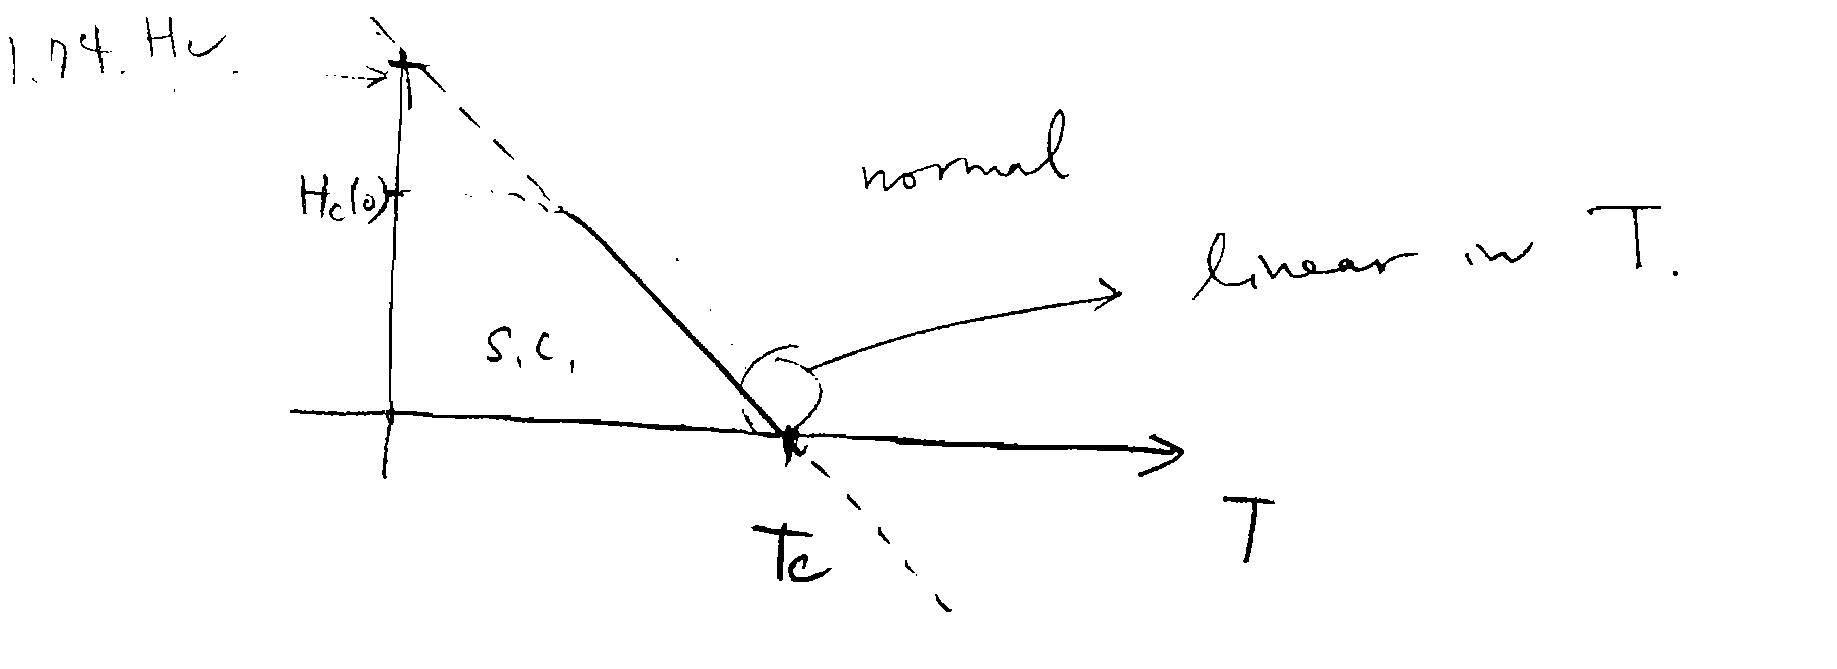
\includegraphics[width = 4.5cm]{6-l2.png}
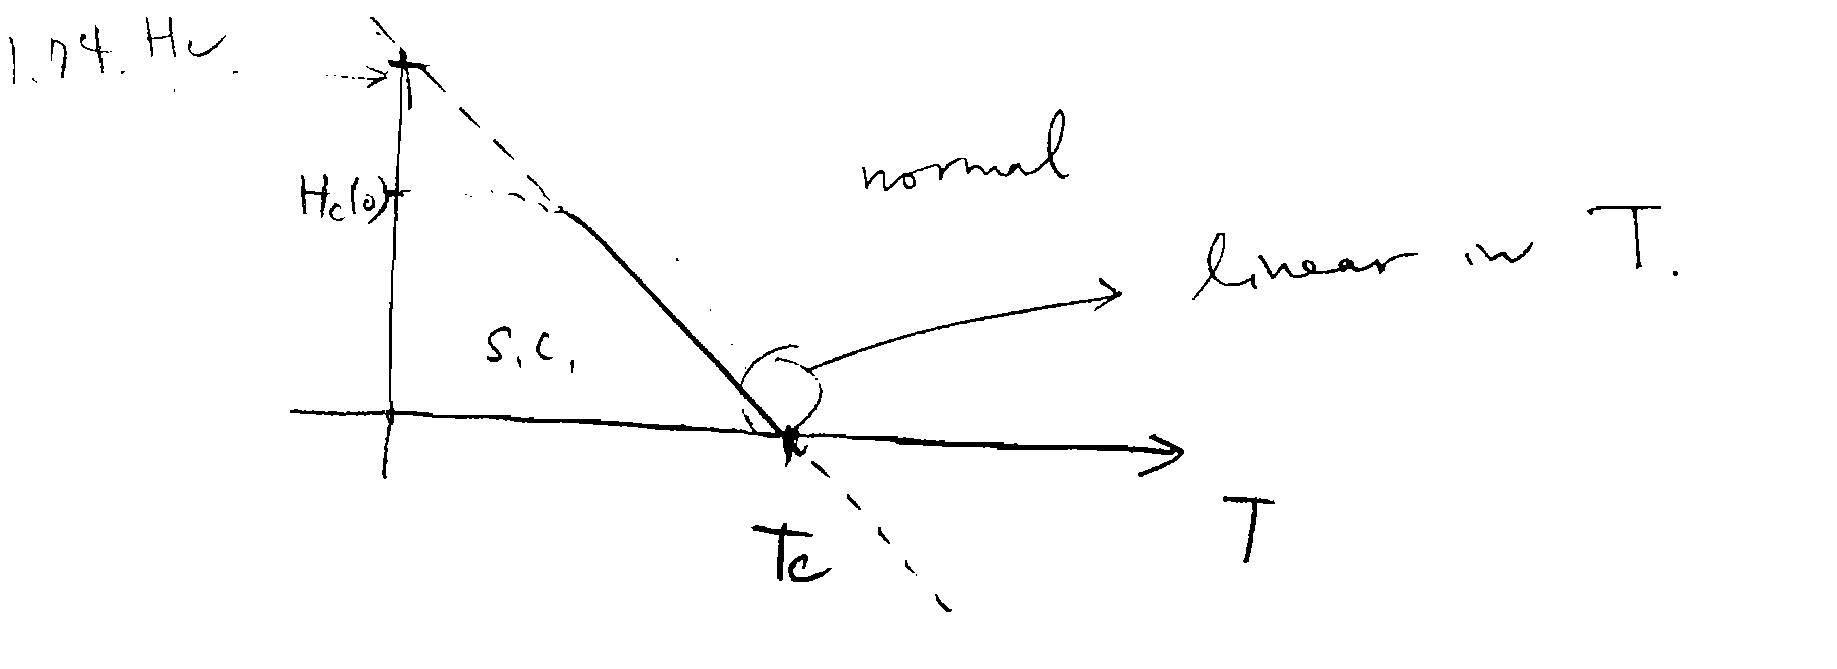
\includegraphics[width = 4.5cm]{6-l1.png}
\end{wrapfigure}



For $T-T_c\ll T_c$, we have

\[H_c(T)=H_c(0)e^\gamma \left[\frac{8}{7\zeta(3)}\right]^{1/3}\left(1-\frac{T}{T_c}\right) \]

From $\Omega_S(T)$ thus obtained, we can also derive the temperature dependence of the sprcific heat:

\[E_S=-T^2\frac{\partial}{\partial T}\left(\frac{\Omega_S}{T}\right),\quad C_S=\left(\frac{\partial E_S}{\partial T}\right)_V \]

Due to the gap in the Bogoliubov excitations, the specific heat at $T\ll T_c$ exhibits the thermal activation form:

\[\frac{C_S}{V}\deq 2N(0)\Delta_0 k_B\sqrt{2\pi}\left(\frac{\Delta_0}{k_B T}\right)^{3/2}e^{-\Delta_0/K_bT},\quad for\quad T\ll T_c \]


